\section{2020 年 12 月 6 日答疑记录}

\subsection{图形变换}

先考虑函数 $y=f(x)$ 与 $y=f(x+1)$ 的图形. 因为点~$A(n,f(n))$ 满足 $y=f(x)$ (此时 $x=n$), 而点~$A'(n-1,f(n))$ 满足 $y=f(x+1)$ (此时 $x=n-1$), 且点~$A$ 向左平移一个单位长度可得点~$A'$, 所以将 $y=f(x)$ 图形上的所有点向左平移一个单位长度可得 $y=f(x+1)$ 的图形.

再考虑函数 $y=f(x)$ 与 $y=f(x)+1$ 的图形. 因为点~$B(n,f(n))$ 满足 $y=f(x)$ (此时 $x=n$), 而点~$B'(n,f(n)+1)$ 满足 $y=f(x+1)$ (此时 $x=n$), 且点~$B$ 向上平移一个单位长度可得点~$B'$, 所以将 $y=f(x)$ 图形上的所有点向上平移一个单位长度可得 $y=f(x)+1$ 的图形.

设 $a>0$, 由同样的分析可以知道, 
\[\begin{aligned}
    &\text{向左平移 $a$ 个单位长度:}\ f(x)\rightarrow f(x+a);\\
    &\text{向右平移 $a$ 个单位长度:}\ f(x)\rightarrow f(x-a);\\
    &\text{向上平移 $a$ 个单位长度:}\ f(x)\rightarrow f(x)+a;\\
    &\text{向下平移 $a$ 个单位长度:}\ f(x)\rightarrow f(x)-a.
\end{aligned}\]
以上结论可以简记为 ``左加右减, 上加下减''. 示意图如下($a>0$):

    \begin{center}
        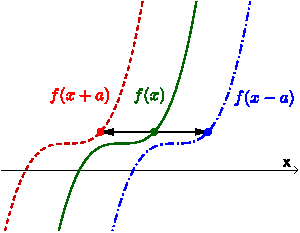
\includegraphics[scale=1]{2020-1215-1900-crop}\qquad
        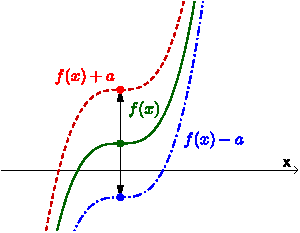
\includegraphics[scale=1]{2020-1215-1910-crop}
    \end{center}

注意, 这些结论均是对 $x$ 或 $f(x)$ (即 $y$) 的整体变换. 例如 $f(2x)$ 的图形往左平移 $1$~个单位长度, 得到 $f(2(x+1))$ 即 $f(2x+2)$ 的图形; 而由 $f(3x)$ 的图形要得到 $f(3x-1)$ 的图形, 需将前者往右平移 $\dfrac13$~个单位长度.

接着考虑函数 $y=f(x)$ 与 $y=-f(x)$ 的图形. 因为点~$C(n,f(n))$ 满足 $y=f(x)$ (此时 $x=n$), 而点~$C'(n,-f(n))$ 满足 $y=f(x+1)$ (此时 $x=n$), 且点~$C$ 与 $C'$ 关于 $x$~轴对称, 所以作 $y=f(x)$ 图形上的所有点关于 $x$~轴的对称点可得 $y=-f(x)$ 的图形 (两个图形上对应点横坐标相同, 纵坐标互为相反数, 简记为 ``上下翻转''). 类似地, 作 $y=f(x)$ 图形上的所有点关于 $y$~轴的对称点可得 $y=f(-x)$ 的图形 (两个图形上对应点横坐标互为相反数, 纵坐标相同, 简记为 ``左右翻转''). 示意图如下:

    \begin{center}
        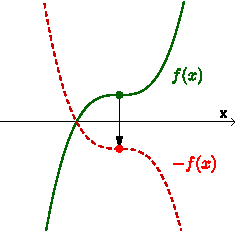
\includegraphics[scale=1]{2020-1215-1920-crop}\qquad
        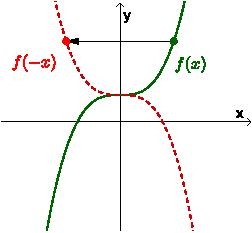
\includegraphics[scale=1]{2020-1215-1930-crop}
    \end{center}

上述六种图形变换可以叠加. 例如, $f(x)$ 的图形先上下翻转可得 $-f(x)$ 的图形, 再左右翻转可得 $-f(-x)$ 的图形; $f(x)$ 的图形先左右翻转可得 $f(-x)$ 的图形, 再向右平移 $4$ 个单位长度 (将 $x$ 替换为 $x-4$) 可得 $f(4-x)$ 的图形.

\begin{example}
    已知 $f(x)=\begin{cases}
        \dfrac12 x,& -2\leqslant x\leqslant 0,\\
        -x^2+2x,& 0<x\leqslant 2,
    \end{cases}$ 画出下列函数的图形:
    
    (1) $f(x)$;\qquad (2) $f(x-2)$;\qquad (3) $-f(x)$;\qquad 
    (4) $f(-x)$;\qquad (5) $-f(-x)$.
\end{example}
\begin{solution}
    各函数图形依次如下:
    
    \begin{center}
        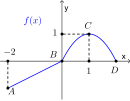
\includegraphics[scale=1.2]{2020-1215-1940-crop}\qquad
        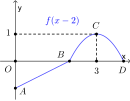
\includegraphics[scale=1.2]{2020-1215-1950-crop}\qquad
        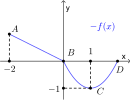
\includegraphics[scale=1.2]{2020-1215-2000-crop}
    \end{center}
    
    \begin{center}
        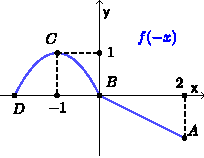
\includegraphics[scale=1.2]{2020-1215-2010-crop}\qquad
        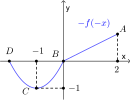
\includegraphics[scale=1.2]{2020-1215-2020-crop}
    \end{center}
\end{solution}

\subsection{恒成立问题}

恒成立问题一般化为值域问题来求解. 例如, 设 $D$ 为函数 $f(x)$ 的定义域, 则
\[\begin{gathered}
    \forall\, x\in D, f(x)\leqslant m\Leftrightarrow f_{\max}\leqslant m,\\
    \forall\, x\in D, f(x)\geqslant m\Leftrightarrow f_{\min}\geqslant m.
\end{gathered}\]

\begin{example}
    已知函数 $f(x)= x^2+ax-b$, 正数 $a$, $b$ 满足 $a+\dfrac4b\leqslant 3$. 若对任意的 $x\in[1,+\infty)$, $f(x)\geqslant 0$ 恒成立, 求 $a$, $b$ 的值.
\end{example}
\begin{solution}
    由题意, 在 $[1,+\infty)$ 上 $f_{\min}\geqslant 0$. 因为 $a$ 为正数, $f(x)$ 的图形的对称轴为 $x=-\dfrac{a}2<0$ 且图形开口向上, 所以此时 $f_{\min}=f(1)=1+a-b$. 因此
    \[\left\{\!\!\begin{array}{l}
        a+\dfrac4b\leqslant 3,\\
        1+a-b\geqslant 0,
      \end{array}\right.\ \text{即}\quad
      \left\{\!\!\begin{array}{l}
        a\leqslant 3-\dfrac4b,\\
        a\geqslant b-1.
      \end{array}\right.\]
    由不等式的传递性, 
    \[3-\frac4b\geqslant b-1,\quad\text{移项整理得}\quad
    0\geqslant (b-2)^2.\]
    因为 $(b-2)^2\geqslant 0$ 恒成立, 所以只能 $(b-2)^2=0$, 即 $b=2$. 回代可知 $a=2$, 所以 $a=b=2$.
\end{solution}